\chapter{Background \& State of the art}

This chapter discusses state of the art in the areas of \emph{\wasm}, \emph{Diversification} and \emph{Runtime Randomization}. We present a summary of the relevant related work and the key concepts and background that we use along with this writing. 
We select the discussed works by their novelty and critical insights to provide automatic diversification. 

In \autoref{sota:wasm} we describe the context in which this dissertation is based, \wasm. We include both usage scenarios for Wasm and its main security issues. In \autoref{sota:diversification} we discuss the main diversification techniques in the wild, we introduce the concept of superoptimization used in this work, and we end the section by highlighting superdiversification as the cornerstone of our contributions are based. In \autoref{sota:randomization} we mention close works to runtime diversification and how diversification can be used to construct resilient binaries. 


\begin{comment}

\todo{Motivate Wasm here}

\todo{Our area is on wasm, compilers, etc}

\todo{The key related work are in the area of X and Y}

\todo{Wasm is not the context ! Define what the context is : compilers, machine code, portable code, Wasm, interpreters, backend, etc. Use background instead of context. Put everythin that is related to the thesis, concepts. }

\todo{Portable code to be distributed}

\end{comment}


\section{\wasm\ overview}
\label{sota:wasm}

%\renewcommand{\lstnumberautorefname}{Line}
\newcommand{\lstnumberautorefname}{Line}
\newcommand{\lineref}[1]{\autoref{#1}}


%\todo{Intro}

%\subsection*{}

% Javascript was first, and then more attempts.
JavaScript is currently used in all modern web browsers to allow client-side scripting. However, due to the complexity of this language, its security flaws and to gain in performance, several alternatives appeared through the years.  For example, Java applets were introduced on web pages late in the 90s to execute Java bytecode in the client side \cite{javaapplet}. Similarly, Microsoft made two attempts with ActiveX in 1996 \cite{activex}, and with Silverlight in 2007 \cite{silverlight}. All these attempts failed to persist or had low adoption, mainly due to security issues and the lack of consensus on the community of browser vendors.

% asm.js and the demonstration of bad language patterns
In 2014, Alon Zakai and colleagues proposed the Emscripten tool \cite{emscripten}. Emscripten used a strict subset of JavaScript, asm.js, to allow low-level code such as C to be compiled to JavaScript. Asm.js was first announced as an LLVM backend \cite{asmjsweb}. This approach came with the benefits of having all the ahead-of-time optimizations from LLVM, gaining in performance on browser clients \cite{asmjs} compared to standard JavaScript code. Asm.js was faster than JavaScript because it limited the language features to those that can be optimized in the LLVM pipeline. Besides, it removed the majority of the dynamic characteristics of the language, limiting it to numerical types, top-level functions, and one large array in the memory directly accessed as raw data. Since asm.js was a subset of JavaScript it was compatible with all engines at that moment. Asm.js demonstrated that client-code could be improved with the right language design and standardization.
% Limitations o0f asm.js and the birth of Wasm
The work of Van Es \etal \cite{EsAsm.js} proposed to shrink JavaScript to asm.js in a source-to-source strategy, closing the cycle and extending the fact that asm.js was mainly a compilation target for C/C++ code. 
%
Nevertheless, JavaScript faces several limitations related to the characteristics of the language. For example, any JavaScript engine requires the parsing and recompiling the JavaScript code which implies a significant overhead.


Following the asm.js initiative, the W3C publicly announced the \wasm\ (Wasm) language in 2017. \wasm\ is a binary instruction format for a stack-based virtual machine and was officially consolidated by the work of Haas \etal \cite{Haas_2017} in 2017. The announcement of \wasm\ marked the first step into the standardization of bytecode in the web environment. Wasm  is designed to be fast, portable, self-contained and secure, and it outperforms asm.js \cite{Haas_2017}. Since 2017, the adoption of \wasm\ keeps growing. For example; Adobe, announced a full online version of Photoshop\footnote{\url{https://twitter.com/Adobe/status/1453034805004685313?s=20&t=Zf1N7-WmzecA0K4V8R69lw}} written in WebAssembly;  game companies moved their development from JavaScript to Wasm like is the case of a full Minecraft version\footnote{\url{https://satoshinm.github.io/NetCraft/}}; and the case of Blazor\footnote{\url{https://dotnet.microsoft.com/en-us/apps/aspnet/web-apps/blazor}}, a .Net virtual machine implemented in Wasm, able to execute C\# code in the browser.

%\todo{Benchmarks}

\subsection{From source to Wasm}

All \wasm\ programs are compiled ahead-of-time from source languages. LLVM includes Wasm  as a backend since release 7.1.0 published in May 2019\footnote{\url{https://github.com/llvm/llvm-project/releases/tag/llvmorg-7.1.0}}, supporting a broad range of frontend languages such as C/C++, Rust, Go or AssemblyScript\footnote{subset of the TypeScript language}. The resulting binary works similarly to a traditional shared library, it includes instruction codes, symbols and exported functions. In \autoref{diagrams:sota:wasm}, we illustrate the workflow from the creation of Wasm  binaries to their execution in the browser. The process starts by compiling the source code program to Wasm  (Step \step{1}). This step includes ahead-of-time optimizations such as optimizations in the LLVM toolchain. 

%To the best of our knowledge, the most complete survey about Wasm  tooling is presented in the Awesome Wasm  (\url{https://github.com/mbasso/awesome-wasm}) repo. It is a cumulative GitHub repo which includes references to articles, papers, books, demos, compilers and engines related to \wasm. 

The step \step{2} builds the standard library for Wasm  usually as JavaScript  code. This code includes the external functions that the Wasm  binary needs for its execution inside the host engine. For example, the functions to interact with the DOM of the HTML page are imported in the Wasm  binary during its call from the JavaScript code. The standard library can be manually written, however, compilers like Emscripten, Rust and Binaryen can generate it automatically, making this process completely transparent to developers.

Finally, the third step (Step \step{3}), includes the compilation and execution of the client-side code. Most of the browser engines compile both the Wasm  and JavaScript codes to machine code. In the case of JavaScript, this process involves JIT and hot code replacement during runtime. For Wasm, since it is closer to machine code, and it is already optimized, this process is a one-to-one mapping. For instance, in the case of V8, the compilation process only applies simple and fast optimizations such as constant folding and dead code removal. Once V8 completes the compilation process, the generated machine code for Wasm does not change anymore and is the same used along all its executions. This analysis was validated by conversations with the V8's development team and by experimental studies in one of our contributions \cite{CROW}.  

\begin{figure}[h]
    \centering
    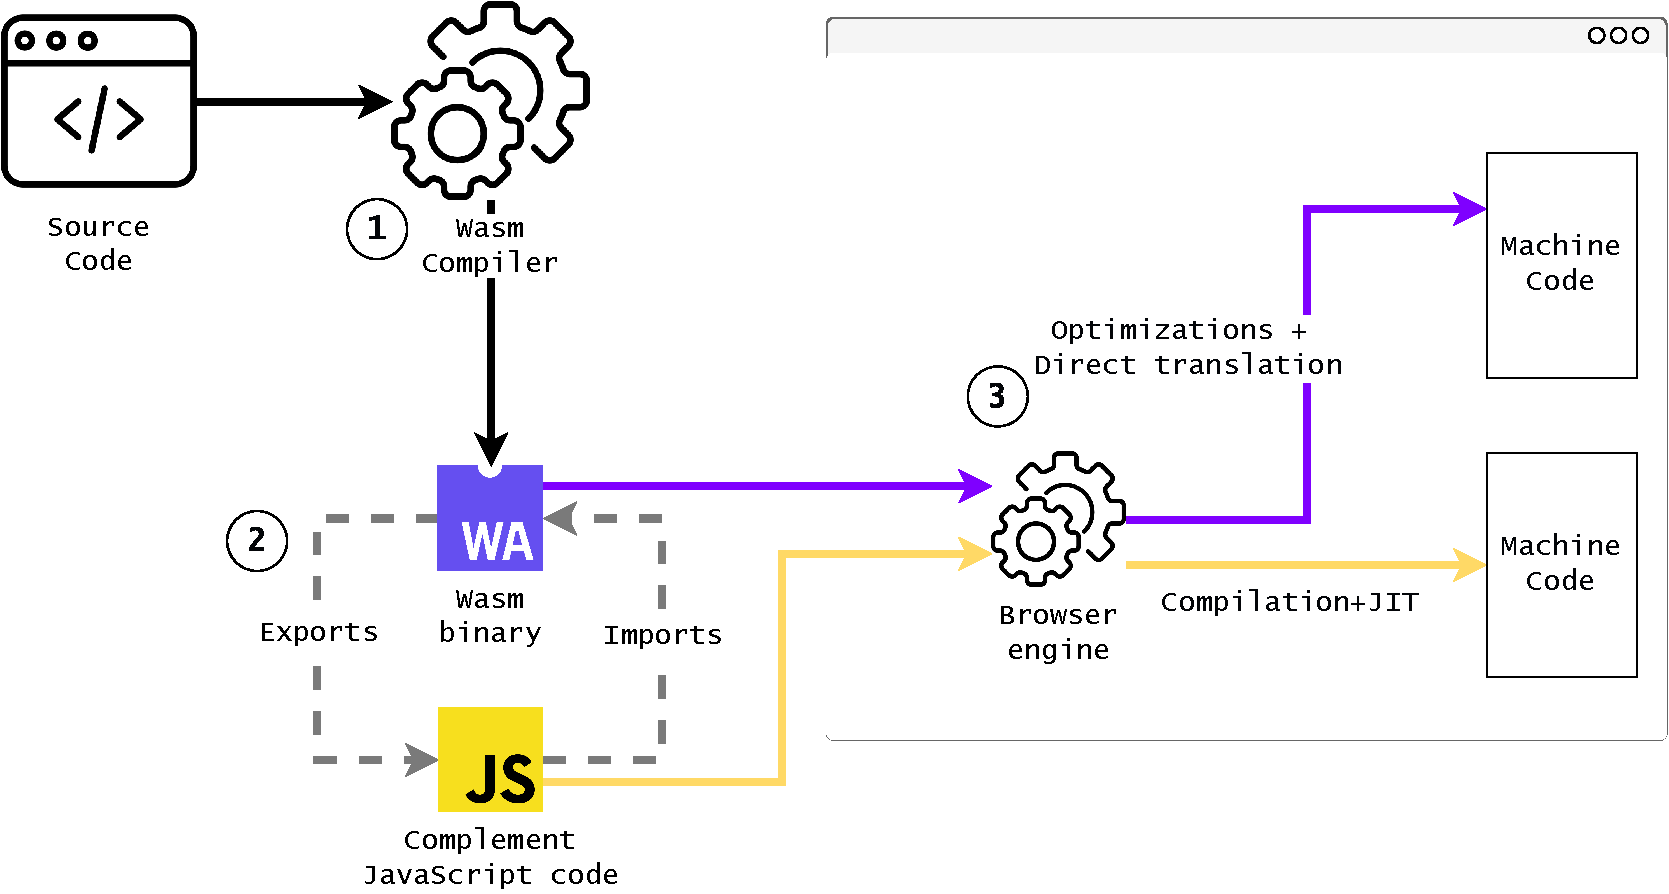
\includegraphics[width=\linewidth]{diagrams/wasm_workflow.pdf}
    \caption{WebAssembly is built, then compiled by the host web browser and finally executed. }
    \label{diagrams:sota:wasm}
\end{figure}

Wasm can execute directly and is platform independent.
Thus, the Internet of Things (IoT) can be seen as the perfect match for \wasm\ \cite{Narayan2021Swivel,Sledge} outside web browsers.
IoT devices are heterogeneous in terms of architecture and platform as the same for Edge computing.
For example, Singh and colleagues \cite{WARDuino2019} proposed a virtual machine for Wasm in arduino based devices.
On the other hand, Cloudflare and Fastly adapted their platforms to provide edge computing services directly with \wasm. 
In these cases, the standard library, instead of JavaScript, is provided by any other language stack that the host environment supports.

In 2019, the Bytecode Alliance \cite{bytecodealliance} proposed the WebAssembly System Interface (WASI) \cite{WASI}. 
WASI is the foundation to build Wasm code outside the browser with a POSIX system interface platform. 
WASI standardizes the adoption of \wasm\ in heterogeneous platforms \cite{bryant2020webassembly}. 

% Talk about benchmarks and performance numbers

%

%\todo{How to obtain WebAssemblybinaries}

%\todo{Browser workflow}

%\todo{How interpreters work, explain the workflow of V8 as it was validated by the V8 compiler developers}

%\todo{Backend workflow}

%\todo{Add a table with tools and interpreters: V8, SpiderMonkey, wasmtime, wasmer, sledge, warduino }


\subsection{WebAssembly specification}

% General description and the introduction of the component, module and section terms
\wasm\ defines its own Instruction Set Architecture (ISA) \cite{wasm_spec}. It is an abstraction close to machine code instructions but agnostic to CPU architectures. Thus, Wasm  is platform independent. The ISA of Wasm  includes also the necessary components that the binary requires to run in any host engine. 
A Wasm  binary has a unique module as its main component. A module is composed by sections, corresponding to 13 types\footnote{\url{https://webassembly.github.io/spec/core/binary/modules.html\#sections}}, each of them with an explicit semantic and a specific order inside the module. This makes the compilation to machine code faster. %The binary format of Wasm  can include custom sections. For example, the work of \todo{Doe} proposed the usage of custom sections to sign binaries for the sake of trusting. 


% Example and intro to the stack
In \autoref{CExample} and \autoref{WASMExample} we illustrate a C program and the Wasm program that results from its compilation. The C function contains: heap allocation, external function declaration and the definition of a function with a loop, conditional branching, function calls and memory accesses. The code in \autoref{WASMExample} shows the textual format for the generated Wasm. The module in this case first defines the signature of the functions (\lineref{tpe1}, \lineref{tpe2}  and  \lineref{tpe3})  that help in the validation of the binary defining its parameter and result types. The information exchange between the host and the Wasm  binary might be in two ways, exporting and importing functions, memory and globals to and from the host engine (\lineref{import1}, \lineref{export1} and \lineref{export2}). The definition of the function (\lineref{func1}) and its body follows the last import declaration at \lineref{import1}. 

% Functions
The function body is composed of local-variable declarations and typed instructions that are evaluated using a virtual stack (Line 7 to Line 32 in \autoref{WASMExample}). Each instruction reads its operands from the stack and pushes back the result. The result of a function call is the top value of the stack at the end of the execution. In the case of \autoref{WASMExample}, the result value of the main function is the calculation of the last instruction, \texttt{i32.add} at \lineref{result}. A valid Wasm  binary should have a valid stack structure that is verified during its translation to machine code. The stack validation is carried out using the static types of Wasm, \texttt{i32} for 32 bits signed integer, \texttt{i64} for 64 bits signed integer, \texttt{f32} for 32 bits float and \texttt{f64} for 64 bits float. As the listing shows, instructions are annotated with a numeric type.

% Example
\begin{code}
    \begin{minipage}[t]{0.45\linewidth}
        \lstset{language=C,caption={Example C function.},
        label=CExample,
        breaklines=true, 
        basicstyle=\small\ttfamily,
        postbreak=\mbox{\textcolor{red}{$\hookrightarrow$}\space},
        escapeinside={(*@}{@*)}
        }
\input{sota/code/code.c}
\end{minipage}\hspace{10mm}
\begin{minipage}[t]{0.46\linewidth}
\lstset{
    language=WAT,
    caption={\wasm\ code  for \autoref{CExample}.},
    style=WATStyle,
    breaklines=true, 
    %stepnumber=0,
    escapeinside={(*@}{@*)},
    numbers=left,
    postbreak=\mbox{\textcolor{red}{$\hookrightarrow$}\space},
    label=WASMExample}
%
\input{sota/code/code.fix.wat}
%\end{lstlisting}
\end{minipage}


%\begin{tikzpicture}[remember picture,overlay]

%\path (2.west) edge[<-, black] (1.west);
%\path (3.west) edge[<-,  black] (4.west);

%\path (6.east) edge[<-, bend right, black] (3.east);
%\path (9.east) edge[<-, bend right, black] (4.east);
%\path (7.east) edge[<-, bend right, black] (8.east);


%\end{tikzpicture}
\end{code}

% Memory, globals and functions
Wasm  manages the memory in a restricted way. A Wasm  module has a linear memory component that is accessed with \texttt{i32} pointers (integer of 32 bits) and should be isolated from the virtual stack. The declaration of the linear data in the memory is showed in \lineref{data}. The memory access is illustrated in \lineref{load}. This memory is usually bound in browser engines to 4Gb of size, and it is only shareable between the process that instantiate the Wasm  binary and the binary itself (explicitly declared in \lineref{mem1} and \lineref{export2}). This ensures the isolation of the execution of Wasm  code. 

Wasm  also provides global variables in their four primitive types. Global variables (\lineref{global1}) are only accessible by their declaration index, and it is not possible to dynamically address them. For functions, Wasm  follows the same mechanism, either the functions are called by their index (\lineref{call}) or using a static table of function declarations. The latter allows modeling dynamic calls of functions (through pointers) from languages such as C/C++, for which the Wasm's compiler is in charge of populating the static table of functions.


In Wasm, all instructions are grouped into blocks, where the start of a function is the root block. Two consecutive block declarations can be appreciated in \lineref{block1} and \lineref{block2} of \autoref{WASMExample}. Control flow structures jump between block boundaries and not to any position in the code like regular assembly code. A block may specify the state that the stack must have before its execution and the result stack value coming from its instructions. Inside the Wasm  binary the blocks explicitly define where they start and end (\lineref{end1} and \lineref{end2}). By design, each block executes independently and cannot execute or refer to outer block codes. This is guaranteed by explicitly annotating the state of the stack before and after the block. Three instructions handle the navigation between blocks: unconditional break, conditional break (\lineref{break1} and \lineref{break2}) and table break. Each break instruction can only jump to one of its enclosing blocks. For example, in \autoref{WASMExample}, \lineref{break1} forces the execution to jump to the end of the first block that starts at \lineref{block1} if the value at the top of the stack is greater than zero.

%We want to remark that de description of Wasm  in this section follows the version 1.0 of the language and not its proposals for extended features. We follow those features implemented in the majority of the vendors according to the Wasm roadmap \cite{wasm_roadmap}. On the other hand we excluded instructions for datatype conversion, table accesses and the majority of the arithmetic instructions for the sake of simplicity.

%There are two types of blocks, regular blocks, used to compound pieces of code for stack validation and loops. A loop block manages iterations, the only difference between this to blocks is that the breaking instruction jumps to the end of the block in the case of loops.

% Self contained loops

% Bound memory, no direct access to the DOM

% Roadmap: threads, SIMD, etc

%\todo{Wasm  Semantics: Add a code listing, explain General layout of a binary, Function and signature, Instructions, Control flow, Memory model, Global model, table model}

%\todo{Add some sentences from the roadmap}

%\todo{Exported function signature allows typing validation before the code is executed}


\subsection{WebAssembly security}

As we described, \wasm\ is deterministic and well-typed, follows a structured control flow and explicitly separates its linear memory model, global variables and the execution stack. This design is robust \cite{WebAssemblySecurity} and makes it easy for compilers and engines to sandbox the execution of Wasm  binaries. Following the specification of Wasm  for typing, memory, virtual stack and function calling,
host environments should provide protection against data corruption, code injection, and return-oriented programming (ROP).

However, implementations in both browsers and standalone runtimes~\cite{Narayan2021Swivel} are vulnerable.
Genkin \etal demonstrated that Wasm  could be used to exfiltrate data using cache timing-side channels \cite{Genkin2018DrivebyKC}.
Moreover, binaries itself can be vulnerable. The work of Lehmann \etal ~\cite{usenixWasm2020} proved that C/C++ source code vulnerabilities can propagate to Wasm  such as overwriting constant data or manipulating the heap by overflowing the stack. Even though these vulnerabilities need a specific standard library implementation to be exploited, they make a call for better defenses for \wasm. 
Recently, Stiévenart and colleagues demonstrate that C/C++ source code vulnerabilities can be ported to Wasm \cite{DeRoover2022}.
% Current proposals
Several proposals for extending \wasm\ in the current roadmap could address some existing vulnerabilities. For example, having multiple memories\footnote{\url{https://github.com/WebAssembly/multi-memory/blob/main/proposals/multi-memory/Overview.md}} could incorporate more than one memory, stack and global spaces, shrinking the attack surface. However, the implementation, adoption and settlement of the proposals are far from being a reality in all browser vendors\footnote{\url{https://webassembly.org/roadmap/}}. 
% In fact, according to the work of Hilbig \etal \cite{Hilbig2021AnES}, the artificial variants created with one of our works contribute to the half of executable and available \wasm\ binaries in the wild.


\section{Diversification and Superdiversification}
\label{sota:diversification}
%\todo{https://www.sciencedirect.com/science/article/pii/S0950584918301484?via\%3Dihub Diversification and obfuscation techniques for software security: A systematic literature review}


\todo{Draw landscape. Emphasis on why for security, sidechannels, etc.}

\todo{Check nicos How to in background related to diversity.}

Program diversification approaches can be applied at different stages of the development pipeline. This section analyzes the related works for both static and dynamic diversification. Besides, we motivate superoptimization strategies to provide a "superdiversifier" that uses intermediate solutions to search for optimal programs to provide program variants. Finally, we describe our contribution to the field.

\todo{Searching for software diversity: attaining artificial diversity through program synthesis}

Static diversification consists in synthesizing, building, and distributing different, functionally equivalent binaries to end-users. This aims at increasing the complexity and applicability of an attack against a large population of users~\cite{cohen1993operating}. \todo{Take a look to Building diverse computer systems }
Dealing with code-reuse attacks, Homescu \etal~\cite{homescu2013profile} propose inserting NOP instruction directly in LLVM IR to generate a variant with a different code layout at each compilation. 
In this area, Coppens \etal~\cite{coppens2013feedback} use compiler transformations to iteratively diversify software.
Their work aims to prevent reverse engineering of security patches for attackers targeting vulnerable programs.
Their approach continuously applies a random selection of predefined transformations using a binary diffing tool as feedback \citationneeded.
A downside of their method is that attackers are, in theory, able to identify the type of transformations applied and find a way to ignore or reverse them.

% Runtime diversification
Previous works have attempted to generate diversified variants that are alternated during execution.
It has been shown to drastically increase the number of execution traces required by a side-channel attack.
Amarilli \etal~\cite{amarilli2011can} is the first to propose the generation of code variants against side-channel attacks.
Agosta \etal~\cite{agosta2015meet} and Crane \etal~\cite{crane2015thwarting}
modify the LLVM toolchain to compile multiple functionally equivalent variants to randomize the control flow of software,
while Courouss{\'e} \etal~\cite{courousse2016runtime} implement an assembly-like DSL to generate equivalent code at runtime in order to increase protection against side-channel attacks. 


% How to use the compiler
Jackson \etal \cite{jackson} have explored how to use NOP operations inserted during compiling time to statically diversify programs. Another idea \todo{Jackson} is to use the optimization flags of several compilers to generate semantically equivalent binaries out of the same source code. These techniques place the compiler at the core of the diversification technique. However, this approach is limited by the number of available flags in the compiler implementation and because the optimization is applied in all possible places in the code at the same time.


\subsection*{Superoptimization}

The search for optimal algorithms to compute a function is as older as of the first compiler. This problem is commonly solved by using human-written heuristics inside the compiler implementations. However, this solution has limitations. First, the optimizations are applied to small pieces of code and do not consider more complex processes like instruction selections, register allocation, and target-dependent optimizations. Second, the well-known phase ordering problem \cite{phase-ordering-problem}. To solve this problem, Massalin \etal \cite{Massalin1987} proposed a superoptimizer, a statistical method to exhaustively explore all possible program constructions to find the smallest program.
Given an input program, code superoptimization focuses on \emph{searching} for a new program variant that is faster or smaller than the original code while preserving its correctness \cite{bunel_learning_2017}.
The search space for the optimal program is defined by choosing a subset of the machine's instruction set and generating combinations of optimized programs, sorted by length in ascending order. If any of these programs are found to perform the same function as the source program, the search halts. However, the exhaustive exploration approach becomes virtually impossible for larger instruction sets.
Because of this, the paper proposes a pruning method over the search space and a fast probabilistic test to check programs' equivalence.

Apart from recent works in the area of Machine Learning \cite{2021arXiv210913498S}, to the best of our knowledge, there are two main implementations for superoptimizers using two completely different strategies.
Churchill et al. \cite{churchill_sound_nodate} implement STOKE to superoptimize large programs for the  Google Native Client stack. They use a bounded verifier to ensure that every generated optimization goes through all the checks for semantic equivalence. STOKE uses a probabilistic approach, following a Monte-Carlo-Markov-Chain strategy to select code transformations that lead to smaller programs.
On the other hand, Souper \cite{bansal_automatic_nodate} automatically generates smaller programs for LLVM following an exhaustive enumerative synthesis. Souper finds subexpressions at the LLVM function level and builds all possible expressions from all the instructions that are no larger than the original subexpression. When Souper finds a replacement, it uses an SMT solver \cite{SMT_solver} to verify the semantic equivalence with the original program. 
Superoptimization is more expensive than traditional optimization heuristics in compilers yet, provides more profound and more robust code transformations.


\subsection*{Superdiversification and statement of novelty}

While finding optimized code, the idea and the implementations of superoptimization discard intermediate solutions that are semantically equivalent to the original program. The discarding of intermediate solutions follows the principle of optimization, finding the best possible program. Jacob \etal~\cite{jacob2008superdiversifier} propose the use of a ''superdiversification'' technique, inspired by superoptimization,
to synthesize individualized versions of programs, their main idea is to keep the intermediate solutions finding the optimal program.
The tool developed by Jacob \etal does not output only the optimal instruction sequence but any semantically equivalent sequences.
Their work focuses on a specific subset of x86 instructions.

In this research, we contribute to the state of the art in artificially creating diversity. While the number of related work for software diversity is enormous, no approach has been applied to the context of \wasm. One of our contributions, CROW, extrapolates the idea of superdiversification for \wasm. CROW works directly with LLVM IR, enabling it to generalize to more languages and CPU architectures, something not possible with the x86-specific approach of previous works.
Furthermore, we conducted a sanity check for diversification preservation, researching to what extent browser compilers do not remove our introduced diversity.

CROW focuses on the static diversification of software. However, because of the specificities of code execution in the browser, this is not far from being a dynamic approach. For example, since \wasm is served at each page refreshment, every time a user asks for a \wasm binary, she can be served a different variant provided by CROW.
It also can be used in fuzzing campaigns \citationneeded to provide reliability. The diversification created by CROW can unleash hidden behaviors in compilers and interpreters.
By generating several functionally equivalent and yet different variants, deeper bugs can be discovered. 
Thanks to CROW, a bug was discovered in the Lucet compiler \footnote{\url{REPO}}.
Fastly acknowledged our work as part of a technical blog post 
\footnote{\url{https://www.fastly.com/blog/defense-in-depth-stopping-a-wasm-compiler-bug-before-it-became-a-problem}} that describes the bug and the patch. 

\section{Runtime diversification}
\label{sota:randomization}

In this section, we highlight past works on runtime strategy for diversification. Besides, we describe and discuss the foundation that supports the composition of diverse yet semantically equivalent programs to enforce security. Finally, we describe our contribution to the field.


A randomization technique creates a set of unique executions for the very same program \cite{bhatkar03}. Seminal works include instruction-set randomization \cite{Kc03,barrantes2003randomized}
to create a unique mapping between artificial CPU instructions and real ones. This makes it very hard for an attacker to ignore the key to inject executable code. This breaks the predictability of program execution and mitigates certain exploits.


Chew, and Song \cite{Chew02mitigatingbuffer} target operating system randomization. They randomize the interface between the operating system and the user applications:
the system call numbers, the library entry points (memory addresses), and the stack placement. All those techniques are dynamic, done at runtime using load-time preprocessing and rewriting. 
Bathkar et al. \cite{bhatkar03,bhatkar2005efficient} proposed three kinds of randomization transformations: randomizing the base addresses of applications and libraries  memory regions, random permutation of the order of variables and routines, and the random introduction of random gaps between objects. 
Dynamic randomization can address different kinds of problems. In particular, it mitigates an extensive range of memory error exploits. 
Recent work in this field includes stack layout randomization against data-oriented programming \cite{aga2019smokestack}, and memory safety violations \cite{lee2021savior}, as well as a technique to reduce the exposure time of persistent memory objects to increase the frequency of address randomization \cite{xu2020merr}.






\subsection*{Moving Target Defense and Multivariant execution}
\label{sota:multivariantex}

% Intro and benefits
Moving Target Defense (MTD) for software was first proposed as a collection of techniques that aim to improve the security of a system by constantly moving its vulnerable components \cite{MTDNationalCyberLaep}.
Usually, MTD techniques revolve around changing system inputs and configurations to reduce attack surfaces. 
This increases uncertainty for attackers and makes their attacks more difficult. 
Ultimately, potential attackers cannot hit what they cannot see. 
MTD can be implemented in different ways, including via dynamic runtime platforms \cite{10.1145/3318216.3363338}. 
Segupta \etal illustrated how a dynamic MTD system \cite{10.5555/3091125.3091155} can be applied to different technology stacks.
Using this technique, the authors illustrated that some CVE related to specific database engines could be avoided.

On the same topic, Multivariant Execution (MVE) can be seen as a Moving Target Defense strategy. In 2006, security researchers at University of Virginia laid the foundations of a novel approach to security that consists in executing multiple variants of the same program. They called this ''N-variant systems'' \cite{cox06}. Bruschi et al. \cite{bruschi2007diversified} and Salamat et al. \cite{salamat2007stopping} pioneered the idea of executing the variants in parallel. Subsequent techniques focus on Multivariant Execution (MVE) for mitigating memory vulnerabilities \cite{lu2018stopping} and other specific security problems incl. return-oriented programming attacks \cite{volckaert2015cloning} and code injection \cite{SalamatJWWF11}.A key design decision of MVE is whether it is achieved in kernel space \cite{osterlund2019kmvx}, in user-space \cite{salamat2009orchestra}, with exploiting hardware features \cite{koning2016secure}, or even through code polymorphism \cite{10.1145/3281662}. Finally, one can neatly exploit the limit case of executing only two variants \cite{maurer2012tachyon,,Kim2015}. Notably,  Davi \etal proposed Isomeron \cite{davi2015isomeron}, an approach  for execution-path randomization. Isomeron simultaneously loads the original program and a variant. While the program is running, Isomeron continuously flips a coin to decide which copy of the program should be executed next at the level of function calls. With this strategy a potential attacker cannot predict whether the original or the variant of a program will execute.


\subsection*{Statement of novelty}
\label{sota:contribs}


Researching on MVE in a distributed setting like the Edge \citationneeded has been less researched. Voulimeneas \etal proposed a multivariant execution system by parallelizing the execution of the variants in different machines \cite{voulimeneas2021dmvx} for the sake of efficiency. Since CROW offers static and runtime diversity for \wasm and its adoption for the Edge and backend executions are becoming security-sensitive fields, we propose an original kind of MVE, MEWE. We generate multiple program variants, which we execute on edge computing nodes. We use the natural redundancy of Edge-Cloud computing architectures to deploy an internet-based MVE.

With MEWE, We contribute to the field of randomization at two stages. First, we automatically generate variants of a given program with CROW, which have different \wasm code and still behave the same. Second, we randomly select which variant is executed at runtime, creating a multivariant execution scheme that randomizes the observable behaviors at each run of the program.



\section{Conclusions}
\label{sota:conclusions}

Software Diversification has been widely researched, not being the case in the \wasm context. With this dissertation, we aim to settle down the foundation to study automatic diversification for \wasm. We contribute to the field of artificial diversity by extending the superdiversifier idea of Jacob \etal \cite{jacob2008superdiversifier}. We empirically demonstrate that CROW provides robust program diversification. Finally, we propose a novel approach of merging program variants to provide multivariant execution. Our
contributions are obtained by following the methodology described in \autoref{chapter:method}. 

%\todo{Wasm and portable code}
%    \todo{How => Why: Motivation, security, reliability}
%\todo{Diversification, Superoptimization and Superdiversification.}
%    \todo{Prexisting => Artificial}
%    \todo{How => Why: Motivation, security, reliability}
%    \todo{Fuzzing (CVE)}
%\todo{Randomization (runtime).}
%    \todo{N-version, Isomeron eg}
%    \todo{How => Why: Motivation, security, reliability}
%\todo{1 - page MEWE and << CROW (Our contributions)}
%    \todo{n-variant}

%\section{CROW}
%\label{section:crow}
